\begin{figure}[h]
    \centering
    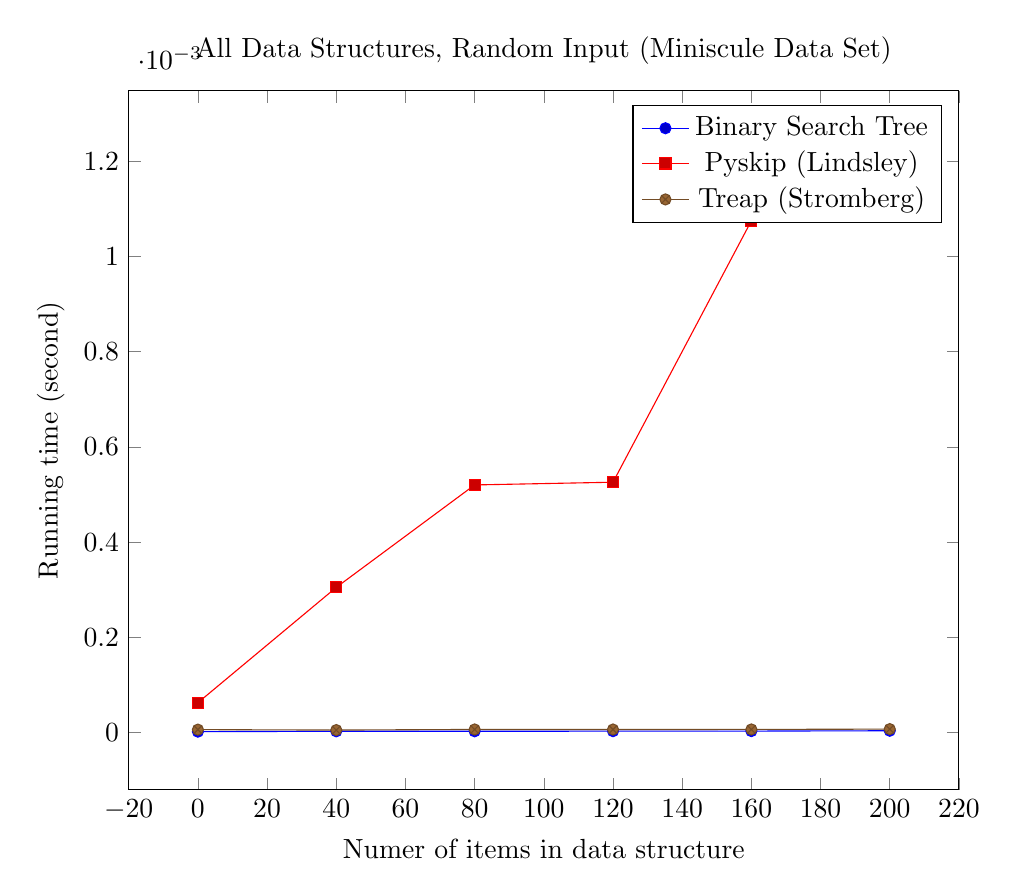
\begin{tikzpicture}
        \begin{axis}[
            xlabel={Numer of items in data structure},
            ylabel={Running time (second)},
            title={All Data Structures, Random Input (Miniscule Data Set)},
            width=\textwidth
        ]
		\addplot coordinates {
			(0, 2.198579958287216e-06)
			(40, 2.9515183001663983e-06)
			(80, 2.9515183001663983e-06)
			(120, 3.2526936369180715e-06)
			(160, 3.3731637716187425e-06)
			(200, 4.095984579822749e-06)
		};
		\addplot coordinates {
			(0, 6.294564538109975e-05)
			(40, 0.00030506049859577004)
			(80, 0.0005201298065701399)
			(120, 0.0005258220204347464)
			(160, 0.0010746839541309963)
			(200, 0.001224940329636405)
		};
		\addplot coordinates {
			(0, 6.445152206485671e-06)
			(40, 5.51150866255623e-06)
			(80, 6.836680144264861e-06)
			(120, 6.716210009560797e-06)
			(160, 6.866797677940184e-06)
			(200, 7.529383418791724e-06)
		};
        \legend{Binary Search Tree, Pyskip (Lindsley), Treap (Stromberg)}
        \end{axis}
    \end{tikzpicture}
    \caption{Average of 10 operations, benchmarked every 40, starting at 0.}
\end{figure}